\documentclass{article}
\usepackage[utf8]{inputenc}
\usepackage{listings}
\usepackage{color} 
\usepackage{titling}
\usepackage{graphicx}
\usepackage{titlepic}

\lstset{
	frame=tb, % draw a frame at the top and bottom of the code block
   	tabsize=4, % tab space width
   	showstringspaces=false, % don't mark spaces in strings
    numbers=left, % display line numbers on the left
    commentstyle=\color{red}, % comment color
    keywordstyle=\color{blue}, % keyword color
    stringstyle=\color{green} % string color
}


\title{\vspace*{\fill} \textbf{COP 290 Assignment 3}
	  \\ {\Large \textbf{Space Invaders}}
	  % \\  \vspace{3mm} 
\includegraphics{ddlogo.png}}
}
\author{
	\vspace{5mm} 
\includegraphics[width=5cm]{logo.png} \\
	 \textbf{Faran Ahmad}\\
	2013CS10220 \vspace{2mm} \\
	\textbf{Kabir Chhabra}\\ 
	2013CS50287 \vspace{2mm} \\
	\textbf{Kartikeya Gupta}\\ 
	2013CS10231 \vspace{2mm} \\
	\textbf{Prateek Kumar Verma}\\ 
	2013CS10246
}
\date{\vspace{3mm} \textbf{March 2015} \vspace*{\fill}}

\begin{document}
	\maketitle

	\newpage

	\tableofcontents

	\newpage

	\section{Objectives}
		Design a game which is :
		\begin{itemize}
			\item Multi-player on-line without a central server.
			\item Has a artificial intelligence component.
			\item Is an action game and not a simple board game.
		\end{itemize}
		\begin{figure}[ht!]
      	\centering
        	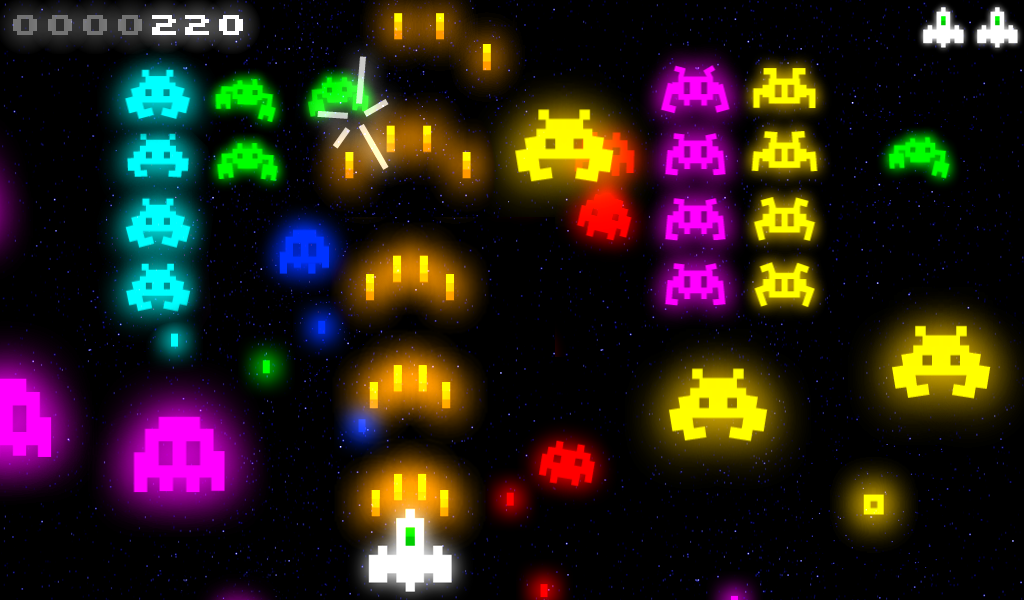
\includegraphics[width=1.0\linewidth]{gameplay.png}
    	\end{figure}
	\section{Overall Design}
		The game which we will build is space invaders. It involves the player controlling a space ship and shooting down aliens. The aliens will fight back with bullets and missiles. The player has a limited number of lives and has to score the maximum in them.
		\begin{enumerate}
			\item The application would be programmed in C++.
			\item The GUI part would involve OpenGL.
			\item UDP sockets will be used for network data transfer.
			\item POSIX threads will be used to run the network and back-end in parallel.
			\item Inter thread synchronization would be done using mutex lock.
		\end{enumerate}

	\section{Sub Components}
		% \begin{enumerate}

			\subsection{Back End}
				The back end has been divided into further sub components to facilitate the development process.
				\subsubsection{Alien}
					This class contains all the information for an alien. The alien will be controlled by artificial intelligence. The level parameter stores the difficulty level which is the quality of AI. There are different types of aliens each with varied number of bullets fired per shot and the number of missiles it has.
					\begin{lstlisting}[language=C++, caption={Class Parameters for Alien}]
class Alien
{
private:
	float XPos;				// X coordinate
	float YPos;				// Y coordinate
	float Angle;			// Orientation angle
	Color ColorOfAlien;		// Color
	int Level;				// AI difficulty level
	int PresentLives;		// Lives left
	int NumberBullets;		// Bullets fired per shot
	int NumberMissiles;		// Number of missiles left
	int AlienType;			// Type
};
					\end{lstlisting}
				\subsubsection{Ship}
					This contains the details for the space ship which are the location, orientation, score, player name etc. If AI has to be active on this player will be determined based on the parameters.
					\begin{lstlisting}[language=C++, caption={Class Parameters for Ship}]
class Ship
{
private:
	float XPos;				// X coordinate
	float YPos;				// Y coordinate
	float Angle;			// Angle
	std::string Name;		// Name of player
	Color ColorOfShip;		// Color of ship
	int Lives;				// Lives left
	int Score;				// Score of player
	int Multiplier;			// Multiplying factor
	int Kills;				// No. of kills
	int Id;					// Player id
	int NumberBullets;		// Bullets fired per shot
	int NumberMissiles;		// Number of missiles left
	int AILevel;			// Level of AI
};
					\end{lstlisting}
				\subsubsection{Color}
					This is a helper class used for storing the color parameters of any object. It has 3 components lying in the range of 0 to 1 for R,G,B values.
					\begin{lstlisting}[language=C++, caption={Class Parameters for Color}]
class Color
{
private:
	float R;				// Value of R component
	float G;				// Value of G component
	float B;				// Value of B component
};
					\end{lstlisting}
				\subsubsection{Bullet}
					Contains all information about bullets and missiles. AI will be active on the missiles. Bullets will travel in straight lines. With each bullet a parameter will store the ship it was fired from so that the score of the player can be incremented appropriately.
					\begin{lstlisting}[language=C++, caption={Class Parameters for Bullet}]
class Bullet
{
private:
	float XPos;				// X Coordinate
	float YPos;				// Y Coordinate
	float VelX;				// Velocity X
	float VelY;				// Velocity Y
	Color ColorOfBullet;	// Color
	int ShipId;				// Id of ship fired from
	bool TypeAI;			// If AI bullet
	bool TypePlayer;		// Player type
};
					\end{lstlisting}
				\subsubsection{Board}
					The entire information of game-play will be controlled from this. The graphics component will use this to generate the display. The network component will keep this in sync amongst all players.
					\begin{lstlisting}[language=C++, caption={Class Parameters for Board}]
class Board
{
private:
	std::vector<Ship> VectorShips;		// All ships
	std::vector<Bullet> VectorBullets;	// All bullets
	std::vector<Alien> VectorAliens;	// All aliens
	double DimensionPosX;				// Dimensions + x	
	double DimensionPosY;				// Dimensions + y	
	double DimensionNegX;				// Dimensions - x	
	double DimensionNegY;				// Dimensions - y		
};
					\end{lstlisting}
			\subsection{Artificial Intelligence}
				The Artificial Intelligence Component of the project will encompass 3 areas:
				\subsubsection{Aliens}
					The AI for Aliens will deal with:
					\begin{enumerate}
						\item Movement of Aliens to dodge Bullets and aim at the ships.
						\item Shooting accuracy, frequency of shooting and speed of the aliens.
						\item Strategies will be adopted by aliens to make life tough for the ships.
					\end{enumerate}
				\subsubsection{Ships}
					The AI for Ships will be a counterpart for the AI for the Aliens with similar features.
				\subsubsection{Missiles}
					The ships will have special potent missiles which can zone into the target. These will be limited in number. The design of the AI for these missiles includes accelerating in the direction of the target and starting to decelerate at the right point of time so that they reach the target exactly and dont overshoot.  
				\subsubsection{Strategy}
					The strategy of the alien/ship will be based on the concept of finite state machines where the AI will transition between particular states of operation, such as attacking, dodging and fleeing, based on the situation.
				\subsubsection{Difficulty}
					\begin{enumerate}
						\item Against aliens: The Alien class has an object level based on which the efficiency of the aliens will be decided using an equation with parameters for accuracy, speed and frequency, and different modes of operation have different coefficients for the factors.
						\item Against opponents: The ship class has an object called AI level which decides the level of efficiency of the ship. Again, this is decided by a complex equation with parameters for the same and different modes of operation.
					\end{enumerate}
				\subsubsection{Learning for AI}
					This will include making different AI players play against each other to ascertain the defining characteristics of a good AI. They will be made to play against different aliens to ascertain the defining characteristics of efficient aliens.
				\subsubsection{Incorporation}
					The AI files will be designed for Entity Pull systems where the AI system is called when a new frame is rendered.


			\subsection{Graphics}
			% \newline
				\begin{enumerate}
					\item To make the graphics we will use OpenGL primarily. Each of the subcomponents like aliens, ships etc will be made in blender and the object files will be generated. Then these object files would be rendered by OpenGL to generate the display.
					\item The frame rate will be set to 30 fps. Whenever a new frame is rendered, the update functions for AI will be called. The user input will also get incorporated accordingly.
					\item GUI effects will be added when bullets shoot down aliens or ships. This will provide a richer and fuller user experience.
				\end{enumerate}
			\subsection{Network Part}
				We will use the User Datagram Protocol (UDP) to design and implement the network aspect of the assignment. It is a communications protocol that offers a limited amount of service when messages are exchanged between computers in a network that uses the Internet Protocol (IP).
				UDP uses a simple connectionless transmission model with a minimum of protocol mechanism. It has no handshaking dialogs, and thus exposes any unreliability of the underlying network protocol to the user's program. There is no guarantee of delivery, ordering, or duplicate protection. UDP provides checksums for data integrity, and port numbers for addressing different functions at the source and destination of the datagram. UDP is suitable for purposes where error checking and correction is either not necessary or is performed in the application, avoiding the overhead of such processing at the network interface level.
				\subsubsection{Why UDP?}
					Our application is a real-time multi-player video game, thus we need fast transfer of data. As stated above, UDP can be fast but unreliable. Even if some of the packets are lost due to unreliability of UDP, it won't affect much. Things change so fast (i.e. player movement, bullets firing) in the game that it doesn't make sense to resend a lost packet as it will contain old information. 
				\subsubsection{Basic Network Design}
					Our network will work on the basis of following points
						\begin{itemize}
							\item Each player will have two basic threads.
							\item One thread for receiving data from other players.
							\item Second thread for sending data to other players.
						\end{itemize}
					\textbf{We shall be sending data} (i.e. player position, AI components data etc) \textbf{as soon a frame is rendered}. This means that we will send almost 30-60 messages every second and hence the use of UDP is justified.
				\subsubsection{Network Outages}
					In the event of a network outages, we shall replace control of the ship of the lost player with AI of same level. The level of AI would be calculated on the basis of the score just before the player was lost. Once the player reconnects, he will automatically gain control of his lost ship.
				\subsubsection{Peer-to-Peer}
					Each of the player in the game would be exchanging its data with each and every other player. Thus we shall implement a peer-to-peer (P2P) connection.
					To control AI components of the game, we shall be using the concept of a ``temporary server'' or a ``virtual server''. A randomly chosen person will be chosen as the ``temporary server''. This player will act as the AI of the game and will send messages to all the other players accordingly. If a player other than this one disconnects, no change is required. If this player disconnects, another active player will be chosen to act as the ``temporary server''.
				\subsubsection{Basic UDP Functions}
					\begin{itemize}
						\item Socket Creation
							\begin{lstlisting}[language=C++, caption={socket()}]
socket(AF_INET, SOCK_DGRAM, 0)		
//AF_INET for Pv4 Internet protocol
//UDP uses SOCK_DGRAM 
//0 is the protocol
							\end{lstlisting}
						\item When a socket is created with socket(), it exists in a name space (address family) but has no address assigned to it. bind() assigns the address specified by addr to the socket referred to by the file descriptor sockfd. addrlen specifies the size, in bytes, of the address structure pointed to by addr. Traditionally, this operation is called ``assigning a name to a socket''.
							\begin{lstlisting}[language=C++, caption={bind()}]
bind(fd, (struct sockaddr *)&myaddr, sizeof(myaddr))
//fd is the sockfd
//myaddr is the address of the player

							\end{lstlisting}
						\item Receiving data
							\begin{lstlisting}[language=C++, caption={recvfrom()}]
recvfrom(fd, buf, BUFSIZE, 0, (struct sockaddr *)&remaddr, &addrlen)
//fd is the sockfd
//buf is array of characters in which the message will be received
//remaddr is the address of the connection player
							\end{lstlisting}
						\item Sending data
							\begin{lstlisting}[language=C++, caption={sendto()}]
sendto(fd, buf, strlen(buf), 0, (struct sockaddr *)&remaddr, addrlen)
//fd is the sockfd
//buf is array of characters which contains the data to be sent
//remaddr is the address of the sending player
							\end{lstlisting}
					\end{itemize}
% \newline
	\section{Interaction amongst Sub Components}
		% \subsection{enumerate}
			\subsection{Back-end and UI}
				The GUI will use the data structures directly. The ``Board'' class will be available to generate the display on the screen. The user inputs from keyboard and mouse will be used to generate changes in the class object. 
			\subsection{Back-end and Network}
				The back end and network components will run on separate threads. Whenever a frame is rendered the network thread for sending will become active. At the same time all the received messages will get processed and applied in the stored parameters. Locks will be used on the message queue to ensure proper synchronization.
	\section{Testing Of Components}
		% \begin{enumerate}
			\subsection{General Unit Tests}
				% \newline
				\begin{lstlisting}[language=C++, caption={Class Parameters for Test}]
class Test
{
private:
	bool verbose;               //If test is to be conducted
	std::string description;    //String description of the test
	bool isPass;                //Boolean if the test has passed 
	void PrintPassFail(bool);   //Prints the status of the test
};
				\end{lstlisting}

				We will use the aforementioned class ``Test'' to perform unit tests on the different files created. This will ensure that all the functions work correctly against some test cases.

			\subsection{Graphics}
				To test the graphics component, we will create aliens and ships at chosen positions. The positions should change appropriately based on user inputs. Bullets should also be fired from the correct positions. When a bullet hits an alien or a ship, proper GUI effects will be added.
			\subsection{Artificial Intelligence}
				Extensive testing of the AI components will include
				\begin{itemize} 
					\item Making AI players of different levels play against each other to make sure the higher level AI players play better. Making them play against different aliens will ascertain that higher level aliens are difficult to beat.
					\item Performance of AI players against real players will also be tested to determine the ideal AI for an interesting competition.
				\end{itemize}
			\subsection{Network Component}
				Testing of network will be divided into two stages.
					\begin{itemize}
						\item In the first stage, we shall test the basic transfer of data. We shall be about 100 dummy messages from one player to another using a simple for loop. The receiver will record the number of messages received and thus we can determine the percentage of packets dropped.
						\item In the second stage, we shall be test the shifting of the ``temporary server'' from one player to another when the player gets disconnected. In this case, the ``temporary server'' shall be sending dummy messages. We shall connect about three players. After the connection is established, we shall close the application of the ``temporary server''. One of the other two must become the ``temporary server'' and sending of dummy message should be continued.
					\end{itemize}
			\subsection{Overall Testing}
				For overall testing of the game, we will play the game with as many players as possible and verify the smooth functioning of AI and network component. The network for some clients will be shut down suddenly to check if the transitions for the AI and others are smooth.
	\section{Extra Features}
		\subsection{Competitive Multi-player Mode}
			In this multi-player mode, the players will be fighting each other. They will try to shoot each other down. Aliens will not be present in this mode. AI players will be present in this.
		\subsection{3D Game-play}
			The game will be taken to 3D in which the aliens and ships can be viewed in a 3D perspective. The camera position will be adjusted by the user based on input from mouse.
		\subsection{Sound Effects}
			Sound effects will be added for the entire game-play. When bullets are fired or some shoot down takes place, appropriate sounds will be played.
		\subsection{Replacement of Player by AI}
			In case of network failures, the player whose network has gone down will get replaced by an AI player of the same level as the player was. This will ensure completely seamless transition in case of network outages. Once the network comes back on, the player will replace the AI control. 
\end{document}
